%! Author = dmytriim
%! Date = 20.03.2021

\documentclass[a4paper,12pt, titlepage]{article}

\usepackage[utf8]{inputenc}
\usepackage[T2A]{fontenc}

\usepackage[english, ukrainian]{babel}

\usepackage{amsmath,amssymb,mathrsfs}
\usepackage{amsthm}
\usepackage[mathscr]{eucal}
%\usepackage[dvips]{graphicx}
\usepackage[pdftex]{graphicx}
\graphicspath{ {.} }

\usepackage{epstopdf}
\usepackage{epigraph}
\usepackage{csquotes}

%\usepackage[centerlast,small]{caption2}
\usepackage{enumerate}
\usepackage{verbatim}
\usepackage{layout}
\usepackage{cite}
%%% remove comment delimiter ('%') and specify parameters if required
%\usepackage[dvips]{graphics}

\usepackage[unicode]{hyperref}
\tolerance=1000
\hypersetup{colorlinks=true}

\pagestyle{empty}

\usepackage{geometry} % Можливість задавати поля
\geometry{top=15mm}
\geometry{bottom=15mm}
\geometry{left=25mm}
\geometry{right=10mm}

\usepackage{extsizes} % Можливість зробити 14-й шрифт(8pt, 9pt, 10pt, 11pt, 12pt, 14pt, 17pt, 20pt.)
\usepackage{multicol}
\usepackage{listings}

% yaml lstlistings
\newcommand\YAMLcolonstyle{\color{red}\mdseries}
\newcommand\YAMLkeystyle{\color{black}\bfseries}
\newcommand\YAMLvaluestyle{\color{blue}\mdseries}

\makeatletter

% here is a macro expanding to the name of the language
% (handy if you decide to change it further down the road)
\newcommand\language@yaml{yaml}

\expandafter\expandafter\expandafter\lstdefinelanguage
\expandafter{\language@yaml}
{
    keywords={true,false,null,y,n},
keywordstyle=\color{darkgray}\bfseries,
basicstyle=\YAMLkeystyle,                                 % assuming a key comes first
sensitive=false,
comment=[l]{\#},
morecomment=[s]{/*}{*/},
commentstyle=\color{purple}\ttfamily,
stringstyle=\YAMLvaluestyle\ttfamily,
moredelim=[l][\color{orange}]{\&},
moredelim=[l][\color{magenta}]{*},
moredelim=**[il][\YAMLcolonstyle{:}\YAMLvaluestyle]{:},   % switch to value style at :
morestring=[b]',
morestring=[b]",
literate =    {---}{{\ProcessThreeDashes}}3
    {>}{{\textcolor{red}\textgreater}}1
    {|}{{\textcolor{red}\textbar}}1
    {\ -\ }{{\mdseries\ -\ }}3,
}

% switch to key style at EOL
\lst@AddToHook{EveryLine}{\ifx\lst@language\language@yaml\YAMLkeystyle\fi}
\makeatother

\newcommand\ProcessThreeDashes{\llap{\color{cyan}\mdseries-{-}-}}

% end yaml lstlistings

% html
\lstdefinelanguage{HTML5}{
    language=html,
    sensitive=true,
    alsoletter={<>=-},
    otherkeywords={
    % HTML tags
        <html>, <head>, <title>, </title>, <meta, />, </head>, <body>,
        <canvas, \/canvas>, <script>, </script>, </body>, </html>, <!, html>, <style>, </style>, ><
    },
    ndkeywords={
    % General
        =,
        % HTML attributes
        charset=, id=, width=, height=,
        % CSS properties
        border:, transform:, -moz-transform:, transition-duration:, transition-property:, transition-timing-function:
    },
    morecomment=[s]{<!--}{-->},
    tag=[s]
}

% end html

\title{\begin{otherlanguage*}{ukrainian}
           \textbf{Аналітичний звіт \\}
           \textit{
               студента 1 курсу денної форми навчання \\
               факультету комп'ютерних наук та кібернетики \\
               Маматюсупова Дмитрія\\
               на тему ,,SEO-аналіз як метод просування веб-ресурсу в мережі Internet.''}
\end{otherlanguage*}}
\author{\begin{otherlanguage*}{ukrainian} Маматюсупов Дмитрій \end{otherlanguage*}}
\date{\begin{otherlanguage*}{ukrainian} Квітень 2021 \end{otherlanguage*}}

\begin{document}
    \maketitle

    \tableofcontents

    \newpage
    \section{Визначення SEO}
    Наведемо визначення в сайту wikipedia.org на різних мовах. \cite{seo_wiki}
    \begin{multicols}{3}
        \textbf{Українська}
        SEO — процес коригування HTML-коду,
        текстового наповнення (контенту), структури сайту, контроль зовнішніх чинників для відповідності
        вимогам алгоритму пошукових систем, з метою підняття позиції сайту в результатах пошуку
        в цих системах за певними запитами користувачів. Чим вище позиція сайту в результатах пошуку,
        тим більша ймовірність, що відвідувач перейде на нього з пошукових систем,
        оскільки люди зазвичай йдуть за першими посиланнями.


        \columnbreak
        \textbf{Русский}
        SEO — комплекс мероприятий по внутренней и внешней
        оптимизации для поднятия позиций сайта в результатах выдачи поисковых систем по определённым запросам пользователей
        , с целью увеличения сетевого трафика (для информационных ресурсов) и потенциальных клиентов
        (для коммерческих ресурсов) и последующей монетизации (получение дохода) этого трафика.
        SEO может быть ориентировано на различные виды поиска, включая поиск информации, товаров, услуг,
        изображений, видеороликов, новостей и специфические отраслевые поисковые системы.

        \columnbreak
        \textbf{English}
        SEO is the process of improving the quality and quantity of website traffic to a
        website or a web page from search engines.
        SEO targets unpaid traffic (known as "natural" or "organic" results) rather than direct traffic or paid traffic.
        Unpaid traffic may originate from different kinds of searches, including image search, video search, academic search,
        news search, and industry-specific vertical search engines.
    \end{multicols}

    Робимо висновок про те, що головною метою SEO є збільшення трафіку сайту, який надодить з пошукової видачі.
    Також зазначимо, що це досягається в тому числі за допомогою змін HTML коду та є специфічним для конкрентої
    пошукової системи.

    Перед тим як перейти до порівняння SEO з іншими видами просування ресурсу ознайомимось з базовими уроками по SEO
    для того, щоб розуміти як проходить SEO для сайту.
    \section{Google}
    Офіційний ``порадник користувача'' по SEO для пошукової системи відомої під іменем Google наводить такі поради/дії
    для покращення рейтингу сайту.
    \begin{enumerate}
        \item \textbf{Дізнатись чи є сайт в індексі Google.}
        Для цього треба зробити пошук сайту із запитом site:`домен'
        Індекс оновлюється автоматично за допомогою ботів(crawlers).
        \item Для того, щоб заблокувати сканування сторінок використовується файл robots.txt. Приклад:
        \begin{lstlisting}[language=yaml, basicstyle=\small, texcl=true]
# приклад.com/robots.txt
# Сказати Google не обходити URL в кошику та картинки в папці icons
# тому, що вони не є корисними для пошуку.
User-agent: googlebot
Disallow: /checkout/
Disallow: /icons/
        \end{lstlisting}

        \item \textbf{Дайте Google доступ до сторінок в тому вигляді, в якому вони з'являются перед користувачами}
        Не додавати в robots.txt файли, які є необхідними для звичайного перегляду сторінки.
        Для перевірки проблем існує такий інструмент: \href{https://support.google.com/webmasters/answer/9012289}{URL Inspection Tool}
        \item \textbf{Забезпечте показ інформативних заголовків та описів сторінок в результатах пошуку Google}
        Заголовок має звучати природньо та співпадати з наповненям сторінки. Заголовок задається тегом \texttt{title}
    \end{enumerate}
    \item \textbf{Викорустовуйте метатег \texttt{description}}
    Метатег допомогає зрозуміти пошуковій системі про що сторінка. Метатег може бути використаний як опис сторінки.
    Приклад:
    \begin{lstlisting}[language=yaml, basicstyle=\small, texcl=true]
<html>
<head>
...
<meta name="description" content="Brandon's Baseball Cards provides a
large selection of vintage and modern baseball
cards for sale. We also offer daily baseball news and events.">
</head>
<body>
    \end{lstlisting}

    \item \textbf{Налаштувати ієрархічну структуру сайту}
    \item \textbf{Робіть цікаві матеріали}
    Готуйте якісні матеріали без помилок. Додайте інформацію про себе.
    Робіть посилання на джерела.
    \item \textbf{Зробіть свій сайт швидким}
    \item \textbf{Оптимізуйте свій сайт для загрузки на мобільних телефонаї}
    Не будемо далі наводити повний список порад, але зрозуміло, що для Google найбільш важливо точний опис наповнення
    сайта, цікавість .

    \section{SEO для сайту КНУ}
    Задля маленької паузи зробимо аналіз сайту КНУ на предмет його підготовленості з точки зору SEO.
    Реклама університету є у 21 столітті одною з важливих частин керування університетом.
    Багато абітуріентів використовує пошукові системи задля вибору alma mater.


    Аналіз запитів. Важливі факти
    \begin{enumerate}
        \item \textbf{По запиту КНУ} в Google першим в видачі є сайт \href{http://www.knu.edu.ua/}{Криворізького національного університету}.
        Тільки потім йде сайт \href{http://www.univ.kiev.ua/}{КНУ ім. Т. Шевченка.} При цьому він виводиться одразу на двох мовах.
        Цей самий запит англійською із Нідерландського VPN дає вже зовсім не такі втішні результати.
        Сайт з'явився на 4й сторінці видачі та навіть не головна сторінка. Для іногородніх студентів рекомендується робити запит `knu kiev'.
        \begin{figure}
            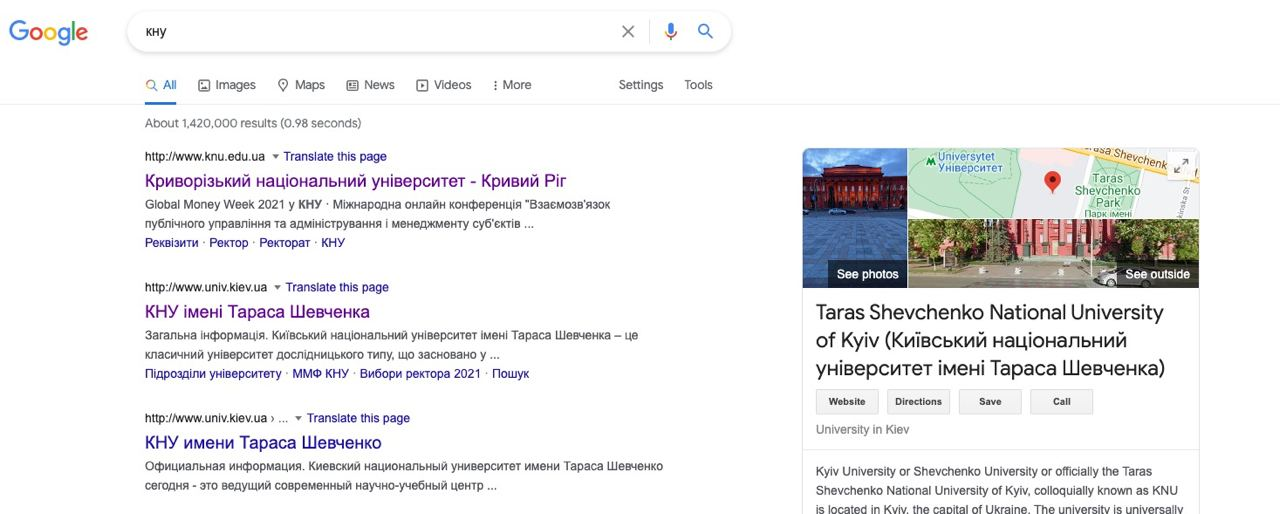
\includegraphics[scale=0.35, left]{knu_search.jpg}
            \caption{Видача Google по запиту КНУ}
        \end{figure}

        \item За допомогою декількох SEO-аналізаторів(наприклад \href{https://sitechecker.pro/}{цей}(64/100), або російськомовний \href{https://seo.analizsaita.online/}{цей}, або \href{https://www.seoptimer.com}{цей}(F) стало зрозуміло,
        що сайту univ.kiev.ua є куди рости. Для початку можна додати редірект на \texttt{https} версію сайту.
    \end{enumerate}

    \section{Порівняльний аналіз SEO та інших методів просування сайту}

    \begin{displayquote}
        З часом однією з основних цілей SEO є те, що ви щодня залучаєте на свій сайт більше людей.
        Не всі вони вам зателефонують, не всі зроблять те, що ви хочете, але якщо ви отримуєте 40, 50, 60 людей на день,
        що є цілком можливо на місцевому ринку, я не маю на увазі Лос-Анджелес або інші великі, але навіть малі міста,
        наприклад, Північна Кароліна або Ебілін, штат Техас. Це цілком можливо.
        Тоді у вас є шанс отримати телефонний дзвінок на день, два телефонні дзвінки на день, подібні речі,
        але це процес, який просто вимагає часу.[\elipsis]
        Давайте порівняємо це з цими іншими способами маркетингу.
        Google Pay-Per-Click, як тільки ви припините платити, ваш трафік миттєво зникає.
        Це як вимкнути електрику.
        Якщо ви робите послугу потенційного клієнта, це продає вам плату за потенційного клієнта, знову ж,
        якщо ви не платите їм, потенційні клієнти зникають і закінчуються.\cite{seo_vs_notseo}
    \end{displayquote}



    \begin{thebibliography}{9}
        \bibitem{seo_wiki}\href{https://en.wikipedia.org/wiki/Search_engine_optimization}{Оптимізація для пошукових систем(англ.)}
        \bibitem{google_seo_guide}\href{https://developers.google.com/search/docs/beginner/seo-starter-guide}{Google посібник по SEO}
        \bibitem{seo_vs_notseo}\href{https://www.speakeasymarketinginc.com/seo-search-engine-optimization-vs-other-web-marketing-methods-which-is-better/}{SEO or Not}
    \end{thebibliography}
\end{document}
